\documentclass[12pt
,headinclude
,headsepline
,bibtotocnumbered
]{scrartcl}
\usepackage[paper=a4paper,left=25mm,right=25mm,top=25mm,bottom=25mm]{geometry} 
\usepackage[utf8]{inputenc}
\usepackage[ngerman]{babel}
\usepackage{graphicx}
\usepackage{multirow}
\usepackage{pdfpages}
%\usepackage{wrapfig}
\usepackage{placeins}
\usepackage{float}
\usepackage{flafter}
\usepackage{mathtools}
\usepackage{hyperref}
\usepackage{epstopdf}
\usepackage[miktex]{gnuplottex}
\usepackage[T1]{fontenc}
\usepackage{mhchem}
\usepackage{fancyhdr}
%\setlength{\mathindent}{0pt}
\usepackage{amssymb}
\usepackage[list=true, font=large, labelfont=bf, 
labelformat=brace, position=top]{subcaption}
\setlength{\parindent}{0mm}

\setlength{\parindent}{0mm}

\pagestyle{fancy}
\fancyhf{}
\lhead{Satellitennavigation\\Übung 1:}
\rhead{Hsin-Feng Ho \\3378849}
\rfoot{Seite \thepage}
\begin{document}
	\begin{titlepage}
		\vspace{\fill}
		\title{\textbf{Satellitennavigation \\ Übung 1}}
		\vspace{5cm}
		\author{Hsin-Feng Ho\\
			3378849}
		\vspace{3cm}
		\maketitle
	\end{titlepage}
	\section{Aufgabe 1}
	\begin{align*}
		\hat{\boldsymbol{a}}=\begin{bmatrix}
			2.23\\2.51
		\end{bmatrix}\qquad\qquad\boldsymbol{Q_{\hat{a}}}=\begin{bmatrix}
		6.29&3.33\\3.33&1.80
	\end{bmatrix}
	\end{align*}
	\subsection{a}
	Einfaches Runden:
	\begin{align*}
	\check{\boldsymbol{a}}=\begin{bmatrix}
		2\\3
	\end{bmatrix}
	\end{align*}
	Boost-strapping (a1):
	\begin{align*}
		\check{a}_1&=\ulcorner a_1 \lrcorner=2\\
		\check{a}_2&=\ulcorner \hat{a}_2-\sigma_{21}\sigma_1^{-2}\left( \hat{a}_1-\check{a}_1\right)  \lrcorner=3\\
			\check{\boldsymbol{a}}&=\begin{bmatrix}
			2\\2
		\end{bmatrix}
	\end{align*}
	Boost-strapping (a2):
\begin{align*}
	\check{a}_2&=\ulcorner a_2 \lrcorner=3\\
	\check{a}_1&=\ulcorner \hat{a}_1-\sigma_{12}\sigma_2^{-2}\left( \hat{a}_2-\check{a}_2\right)  \lrcorner=1\\
	\check{\boldsymbol{a}}&=\begin{bmatrix}
		1\\3
	\end{bmatrix}
\end{align*}
\subsection{b}
Z-Transformaiton:
\begin{align*}
	\boldsymbol{Q}^{(1)}&=\boldsymbol{Q_{\hat{a}}}\\
	\alpha_1&=-\ulcorner\sigma_{12}/\sigma^2_1\lrcorner=-1\\
	\boldsymbol{Z}_1&=\begin{bmatrix}
		\alpha_1&1\\1&0
	\end{bmatrix}=\begin{bmatrix}
	-1&1\\1&0
\end{bmatrix}
\end{align*}
Iteration bis $\alpha_i=0$:
\begin{align*}
	\alpha_i&=-\ulcorner\sigma_{12}\left( i\right) /\sigma^2_1\left( i\right)\lrcorner\\
	\boldsymbol{Z}_i&=\begin{bmatrix}
	\alpha_i&1\\1&0
	\end{bmatrix}\\
\boldsymbol{Q}^{(i+1)}&=\boldsymbol{Z}_i\boldsymbol{Q}^{(i)}\boldsymbol{Z}_i^{T}\\
	\boldsymbol{Z}&=\boldsymbol{Z}_{i}\boldsymbol{Z}_{i-1}\dots\boldsymbol{Z}_1
\end{align*}
Nach Iteration:
\begin{align*}
	\boldsymbol{Z}_4&=\begin{bmatrix}
		0&1\\1&0
	\end{bmatrix}\\
\boldsymbol{Q}_4&=\begin{bmatrix}
	0.1700&0.0700\\0.0700&1.400
\end{bmatrix}\\
\boldsymbol{Z}&=\begin{bmatrix}
	-1&2\\-2&3
\end{bmatrix}\\
\boldsymbol{z}&=\boldsymbol{Z}\hat{a}=\begin{bmatrix}
	2.79\\3.07
\end{bmatrix}\\
\check{\boldsymbol{z}}&=\ulcorner\boldsymbol{z}\lrcorner=\begin{bmatrix}
	3\\3
\end{bmatrix}
\end{align*}Rücktransformation:
\begin{align*}
\check{\boldsymbol{a}}=\boldsymbol{Z}^{-1}\boldsymbol{\check{z}}=\begin{bmatrix}
	3\\3
\end{bmatrix}
\end{align*}
\subsection{c}
Induktionsprinzip:
\begin{align*}
	\boldsymbol{Z}_1=\begin{bmatrix}
		\alpha_1&1\\1&0
	\end{bmatrix}\\
det(\boldsymbol{Z}_1)=-1
\end{align*}
Induktionshypothese:
\begin{align*}
	det(\boldsymbol{Z}_i)=\pm1
\end{align*}
Induktionsschluss:
\begin{align*}
	det(\boldsymbol{Z}_{i+1})=det(\begin{bmatrix}
		\alpha_{i+1}&1\\1&0
	\end{bmatrix}\begin{bmatrix}
	a&b\\c&d
\end{bmatrix})=ab\alpha_{i+1}+bc-ab\alpha_{i+1}-ad=bc-ad=-det(\boldsymbol{Z}_i)
\end{align*}
Damit ist $det(\boldsymbol{Z})=\pm1$ wahr.\\\\
Da $\alpha_i$ aus Runden ergibt, muss es ganzzahlig sein. Die Multiplikationen von Ganzzahlen sollen ebenfalls ganzzahlige Matrix ergeben.
\section{Aufgabe 2}
\subsection{a}
Methode 3: integer rounding method:
\begin{align*}
\check{\boldsymbol{a}}=\begin{bmatrix}
	-25309635\\-19534861\\-23169347\\-18022786\\2384870\\1896465\\-19226459\\-14940096\\-9005552\\-7028940
\end{bmatrix}
\end{align*}
Methode 4: integer booststrapping method:
\begin{align*}
	\check{\boldsymbol{a}}=\begin{bmatrix}
		-25309635\\-19534861\\-23169347\\-18022786\\2384870\\1896465\\-19226459\\-14940096\\-9005552\\-7028940
	\end{bmatrix}
\end{align*}
Methode 2: ILS method based enumeration in search
\begin{align*}
	\check{\boldsymbol{a}}=\begin{bmatrix}
		-25309635&-25309631\\-19534861&-19534858\\-23169347&-23169347\\-18022786&-18022786\\2384870&2384879\\1896465&1896472\\-19226459&-19226458\\-14940096&-14940095\\-9005552&-9005552\\-7028940&-7028940
	\end{bmatrix}
\end{align*}\begin{align*}
 \text{sqnorm}=\begin{bmatrix}
 	1.95&28.7662
 \end{bmatrix}
\end{align*}
\subsection{b}
\begin{align*}
	\tau_0=1.95/28.7662=0.0678<0.5
\end{align*}
\section{Aufgabe 3}
\begin{figure}[H]
	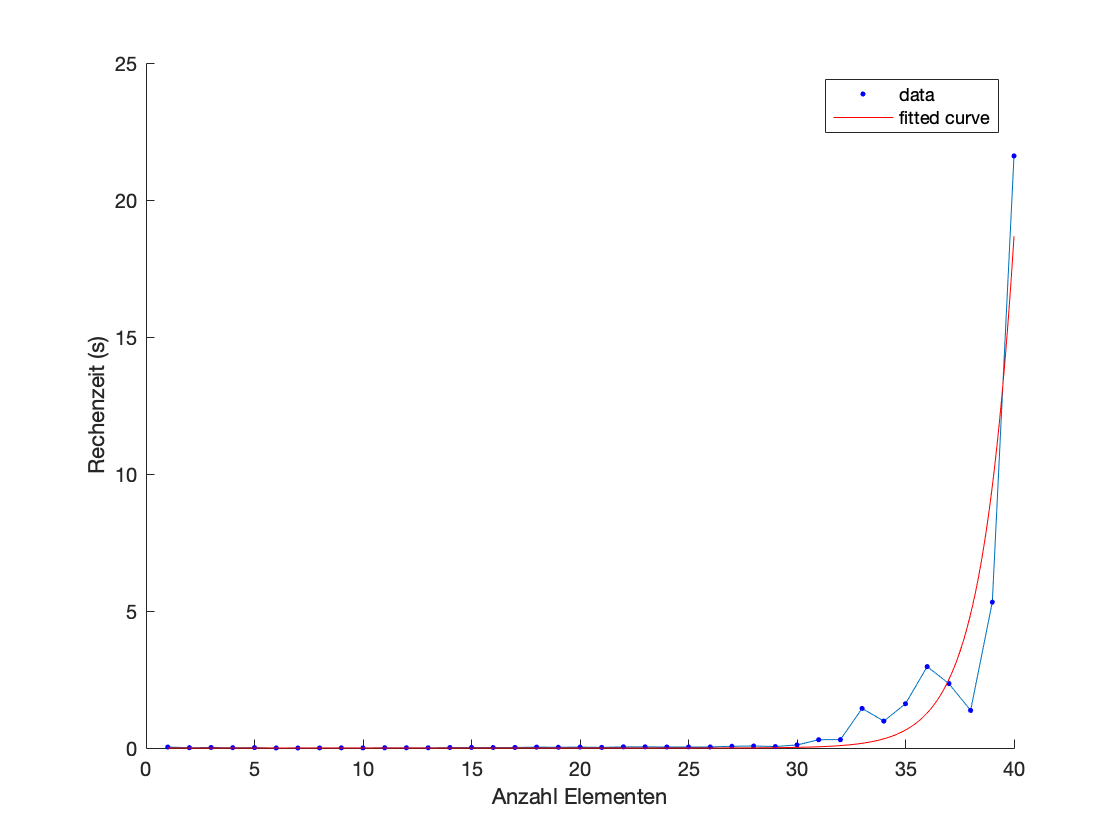
\includegraphics[width=15cm]{figure}
\end{figure}
MacBook Pro 2.3 GHz Dual-Core Intel i5 8GB RAM
\end{document}